\chapter{Context of the work}
\minitoc
\newpage

\setcounter{secnumdepth}{0} % Set the section counter to 0 so next section is not counted in toc
% ----------------------- Introduction ----------------------- %
\section{Introduction}
This chapter introduces the general context of this report. We start by
stating the problem which led to the realization of the project. Then we suggest a solution to these problems. Finally, we define the methodology we've followed to carry out our work.

\setcounter{secnumdepth}{2} % Resume counting the sections for the toc with a depth of 2 (Sections and sub-sections)
% ----------------------------------- SECTIONS (v) ----------------------------------- %
% ----------------------- Stating the problem ----------------------- %
\section{Stating the problem}
In this context, our focus is on the following question: "What set of messages should be sent to a lead to maximize their conversion rate?" This question encapsulates the core challenge faced by the marketing team, namely the ability to tailor communication strategies that resonate with leads. Our main goal, in the end is to generate more leads and increase the conversion rate.

% ----------------------- Assessment of the case ----------------------- %
\section{Proposed solution}
To address the defined challenge, we propose a solution that makes use of machine learning methodologies. Leveraging a diverse dataset extracted from our SaaS platform, encompassing information about campaigns, leads, messages, records, and users, our approach aims to unravel patterns and insights that lead to effective lead engagement. By recommending the most suitable messages, our solution seeks to enhance the efficiency of the lead generation process.

% ----------------------- Assessment of the case ----------------------- %
\section{Development methodology}
\subsection{Kanban methodology}
Kanban is all about visualizing your work, limiting work in progress, and
maximizing efficiency (or flow). Kanban teams focus on reducing the time a
project takes from start by using a Kanban board to continuously improve
their flow of work. To explain more in details, Kanban is based on a con-
tinuous workflow structure that keeps teams nimble and ready to adapt to
changing priorities. Work items —represented by cards— are organized on
the board where they flow from one stage of the workflow or column to the
next. Common workflow stages are To Do, In Progress, In Review, and
Done.

\begin{figure}[H]
    \centering
    \makebox[\textwidth]{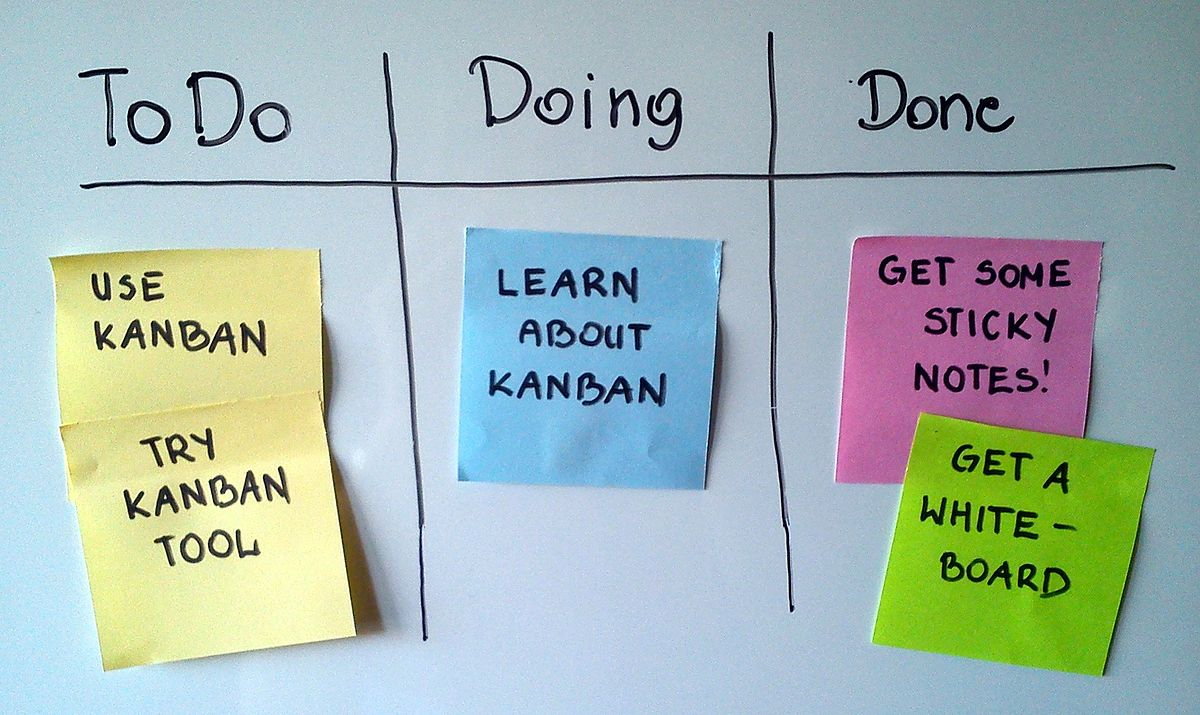
\includegraphics[width=\linewidth]{src/assets/images/simple-kanban-board.jpg}}
    \caption{ILG project Kanban board}
    \label{fig:ilg-project-kanban-board}
\end{figure}

\subsection{The choice for our project}
Since this project is quite susceptible to change, we decided to use the Kanban methodology. The latter is very flexible and allows us to adapt to the changes that may occur. This means delivering the project in a shorter time.

% ----------------------------------- SECTIONS (^) ----------------------------------- %

\setcounter{secnumdepth}{0} % Set the section counter to 0 so next section is not counted in toc
% ----------------------- Conclusion ----------------------- %
\section{Conclusion}
In this chapter, we have presented the general context of this report. We have also stated the main problem and proposed a solution to it. In the next chapter, we will explore the datasets that we have access to and the data exploration and preprocessing steps that we did.
